\section{Fundamentals of EELS}
\label{sec:eels}

Realizing the full potential of any material requires knowing its 
precise electronic, structural and chemical information at high spacial resolution.
%
One way to achieve this is by means of electron energy loss spectroscopy (EELS).
%
EELS is a method used in combination with 
transmission electron microscopy (TEM), which analyses the 
energy distribution of initially monoenergetic electrons after
they have interacted with a specimen~\cite{Egerton:1996}. 
%
In this chapter, we present an introduction to the basics
of EELS, followed by an overview of energy loss spectra and 
the limitations of the technique.\\

Electron energy loss spectroscopy was developed by James Hillier and R.F. Baker in 
the mid-1940s~\cite{Hillier:1944},
but it was only becoming more widespread in research in the 1990s 
due to improvements in microscope instrumentation. 
%
Since modern instrumentation became widely available in laboratories in the
mid-1990s, the scientific developments regarding electron microscopes grew rapidly.
%
Especially since the introduction of modern aberration correctors
and monochromated electron sources, energy resolutions of 100 meV
or even higher could be achieved~\cite{Rose:2008},
which enabled measurements of single (columns of) atoms. 

Transmission electron microscopy can provide structural information 
with excellent spatial resolution down to atomic dimensions. 
%
These compositional data can be supplemented by chemical information 
from the same specimen region, obtained using analytical techniques
such as EELS.
%
EELS instrumentation is typically incorporated into a scanning
transmission electron microscope (STEM) or in a conventional TEM (c-TEM).
%
These microscope types use high energy electrons, typically 60 - 300 keV, 
to interrogate the sample. 
%
The transmitted electrons are deflected through a uniform magnetic field 
of the order of 0.01 T, generated by an electromagnet with carefully shaped polepieces. 
%
Electrons that scattered inelastically will stray from the central trajectory, 
giving rise to a greater or lesser deflection angle, 
and are sorted and detected according to their energies. 
%
The existence of different kinetic energies thus results in a fringing 
field at the EELS detector.
%
A schematic illustration of a typical EELS setup is shown in the left panel of Fig.~\ref{fig:EELS}.
%

%%%%%%%%%%%%%%%%%%%%%%%%%%%%%%%%%%%%%%%%%%%%%%%
\begin{figure}[H]
    \centering
    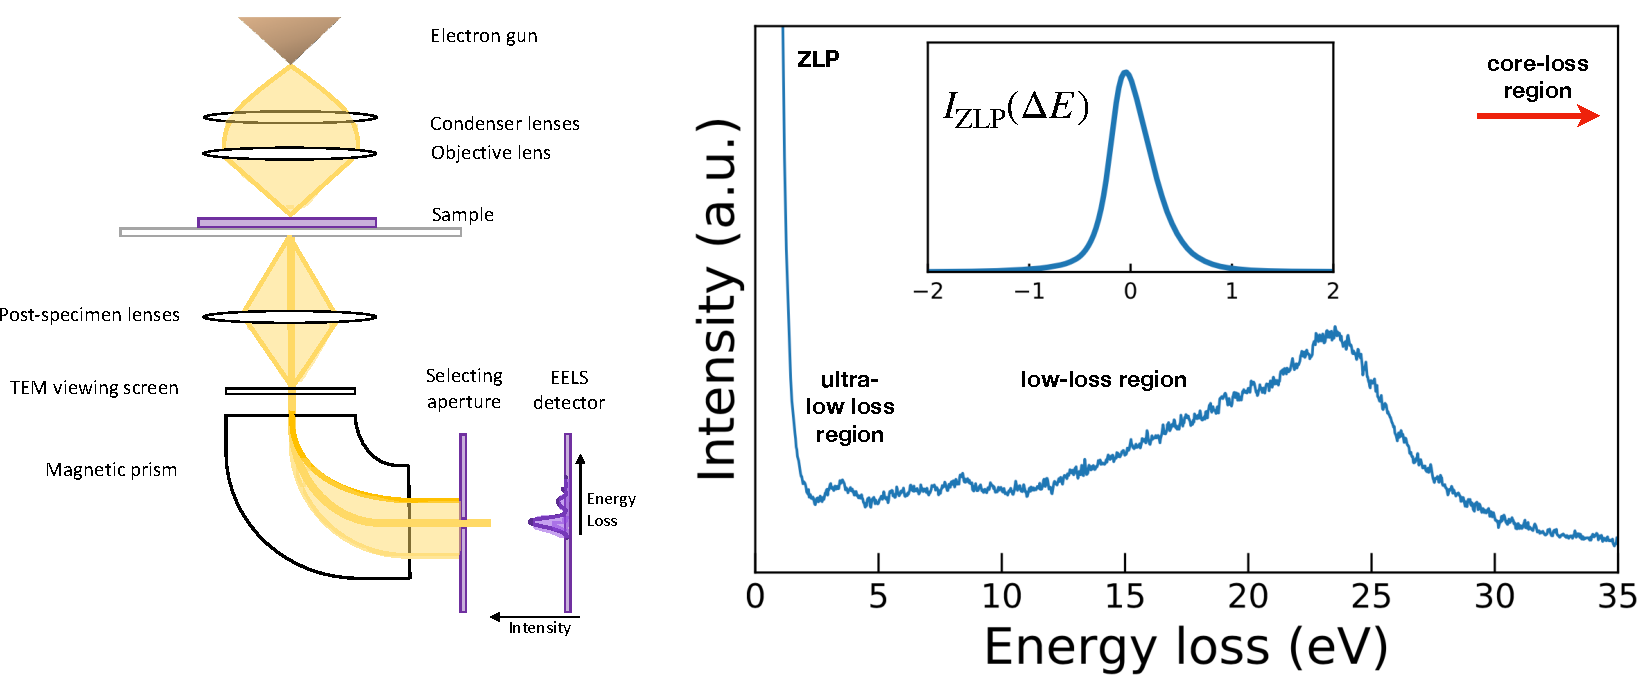
\includegraphics[width=0.97\textwidth]{plots/EELS.pdf}
    \caption{Left: in STEM-EELS, a magnetic
      prism is used to deflect the electron beam after crossing the sample
      so that the distribution of their energy losses $\Delta E$ can be recorded.
      %
      Right: a representative spectrum for $\Delta E \le 35$ eV acquired 
      on a WS$_2$ nanoflower~\cite{SabryaWS2} with
      the inset displaying the corresponding ZLP.
      }
    \label{fig:EELS}
\end{figure}
%%%%%%%%%%%%%%%%%%%%%%%%%%%%%%%%%%%%%%%%%%%%%%%%5

Electron energy loss spectroscopy  provides detailed information about the 
chemical components, bonding, and structure of the specimen.
%
Thanks to recent progress in TEM instrumentation and data acquisition, the EELS technique 
benefits from a combination of both
highly competitive energy (spectral) resolution and spatial resolution.
%
Especially scanning transmission electron microscopy (STEM) equipped with a monochromator 
is extremely useful for high resolution imaging.
%%
The right panel of Fig.~\ref{fig:EELS} displays
a representative EELS spectrum in the region $\Delta E \le 35$ eV, recorded
in one of the WS$_2$ nanostructures presented in~\cite{SabryaWS2},
which will be further discussed later onwards.

\subsection{EEL spectra}
If we are to understand how the features in electron energy loss spectra are produced, 
we must consider how the interaction of the incident electron with the sample 
contributes to the spectrum. 
%
Roughly speaking, EEL spectra can be divided into three main regions.\\

{\bf Zero-loss region.} The first is the zero-loss region, which is centered around $\Delta E=0$
and contains the contributions from electrons that are transmitted without suffering
measurable energy loss.
%
Provided the thickness of the sample is small, the greatest part of the 
incident electron beam transfers through the sample elastically, 
implicating the energy exchange is less than the experimental energy resolution. 
%
A strong and narrow intensity peak around 0 eV loss can be observed called the zero-loss peak (ZLP) or elastic peak. 
The width of the ZLP, typically 0.2-2 eV, reflects the energy distribution of the electron source.

The inset in Fig~\ref{fig:EELS} displays the ZLP, illustrating how nearby $\Delta E\simeq 0$
its magnitude is larger than the contribution from the inelastic interactions
with the sample by several orders of magnitude.
%
This can be explained by the fact that a nucleus is thousands of times more massive than an electron, 
and therefore the energy transfer involved in elastic scattering is usually negligible. 
%
The probability of elastic scattering for a single incident electron 
(per unit solid angle $\Omega$) can to a first approximation be described by 
the differential cross section~\cite{Egerton:1996},
\begin{equation}
    d\sigma_e / d\Omega = \frac{4Z^2/k_0^2T}{(\theta^2 + \theta_0^2)^2}
\end{equation}

where $Z$ is the atomic number, $k_0$ the electron wavenumber, 
and $T$ is not the temperature but the incident electron energy. 
$\theta$ is the scattering angle of the electron of interest, 
and $\theta_0$ represents the angular width of the scattered beam. \\

{\bf Low-loss region.} The second region is the low-loss region or valence region, defined for energy losses
$\Delta E \lsim 50$ eV, which contains information about interactions between the fast incident electrons
and the atoms in the specimen.

The two most fundamental types of collective electronic excitations in solids are plasmons and excitons.
%
In EEL spectra recorded on rather thick specimens, the most prominently observed peaks are plasmon peaks.
%
When an incident electron travels through the crystal lattice, the outer-shell electrons bound to the lattice atoms
are left oscillating, creating a collective of electron excitation modes called  a plasma resonance.
%
This excitation can also be described by means of the creation of a pseudoparticle called a plasmon, 
whose energy depends on the plasmon frequency~\cite{Nerl:2016}.
%
The higher the electron density, the higher the plasmon frequency and therefore the plasmon energy. 
%
Characteristic plasmon-loss peaks appear in the EEL spectra between 5 and 50 eV energy loss, and
can be used to determine the thickness of the specimen, since a higher thickness leads to more
plasmon excitations.

Additionally, the passage of an incident electron can lead to the excitation of a single outer-shell electron.
%
For an insulator or semiconductor, this involves an inter-band transition across the energy bandgap, leaving a hole
behind in the valence band. 
%
The bound state of the electron in the conduction band and electron hole in the valence band is called an exciton.
%
Exciton features appear in the ultra-low-loss region of EEL spectra close to the ZLP, 
characterised by $\Delta E \simeq$ few eV.
%
Here, the contributions of the ZLP and those from the inelastic interactions
with the sample are of the same order of magnitude, and they can be therefore difficultly distinctive~\cite{Abajo:2010}.

When we are dealing with a metal, the higher state can be within the same energy band, corresponding to 
an intra-band transition.
%
Peaks arising from intra-band transition appear very close to the ZLP, with typical energy losses 
below 500 meV.\\

For very thin specimens, the surface and bulk plasmons largely disappear, leaving
interband transitions as the main features in the low-loss regime~\cite{Egerton:1996}.
%
This facilitates the study after the direct bandgap of the material.
%
The  bandgap  refers  to  the  energy  difference between the top of the valence band 
and the bottom of the conduction band and the corresponding peak is expected to appear 
at energy losses where the joint density of states (JDOS) exhibits maxima. 
%
The nature of the bandgap can be either direct or indirect. For direct bandgap materials,
electrons can be directly excited from valence to conduction band. However, 
for indirect band gap materials, a photon or phonon is required to facilitate the transition.
%
For this reason, direct bandgap materials tend to have stronger absorption properties.\\


It has been shown by Bruley and Brown~\cite{Bruley:1987} that for parabolic bands, 
the JDOS probed by the electrons can be described by
\begin{equation}
\label{eq:bandgap}
    \rho(E) = \frac{V}{4\pi^2} \left( \frac{2m^*}{\hbar} \right)^{(3/2)} \alpha \sqrt{E-E_{bg}}
\end{equation}
for a direct band gap, where $m^*$ is the mass of the electrons and holes in the 
valence and conduction band, $E_{bg}$ is the band gap energy and $\alpha$ is the 
convergence angle of the electron beam.
%%
The nature (direct of indirect) and the band gap energy can be deduced 
from the first few eV of the energy-loss function. 
%
From a fit of the band gap onset to Eq.~\ref{eq:bandgap}, 
the value of (1/2) for a direct bandgap switches to (3/2) for an indirect bandgap,
as demonstrated in Fig.~\ref{fig:bandgap}.

\begin{figure}[H]
    \centering
    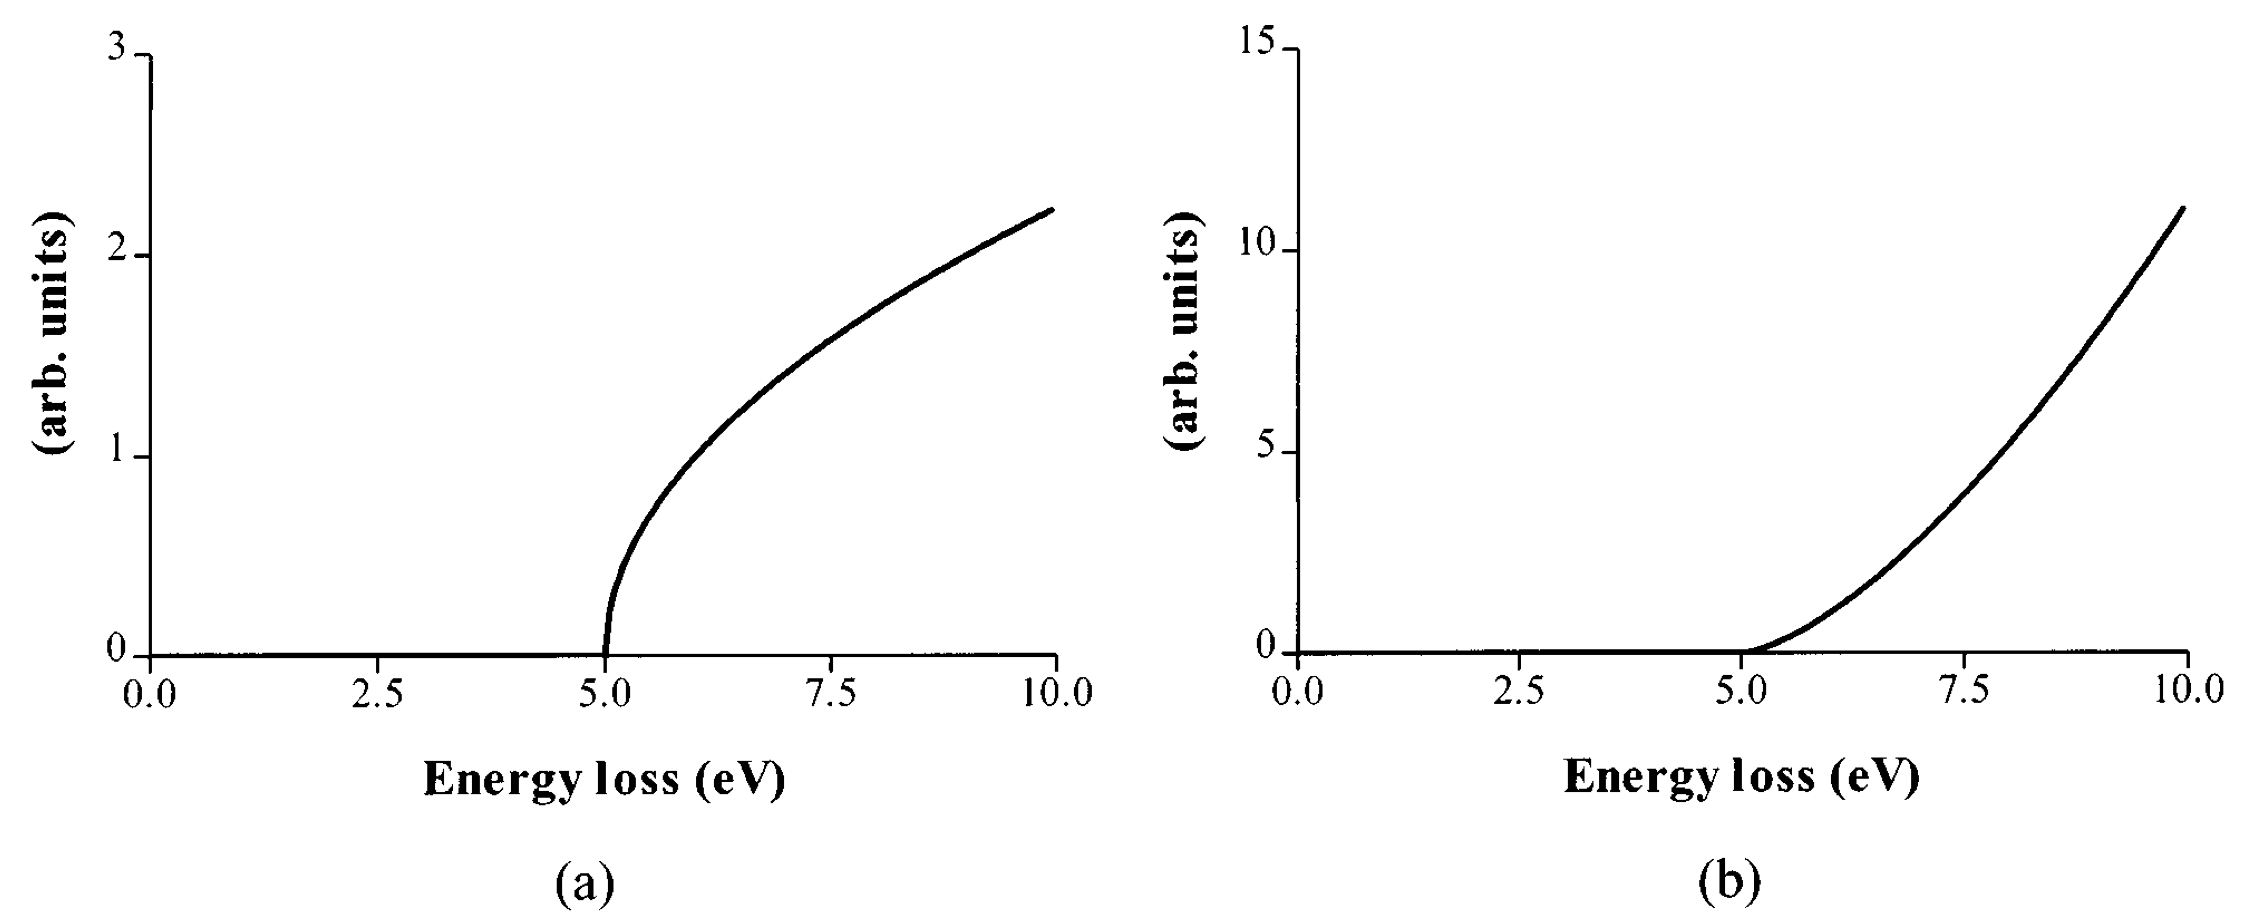
\includegraphics[width=0.8\textwidth]{plots/bandgap.png}
    \caption{Schematic diagrams showing the contributions from the JDOS and matrix elements for (a) direct and (b) indirect transitions. From a fit of the bandgap onset to Eq.~\ref{eq:bandgap}, the power of (1/2) for a direct bandgap switches
    to (3/2) for an indirect transition.
    %
    Retrieved directly from~\cite{Rafferty:1998}.}
    \label{fig:bandgap}
\end{figure}

For materials with a large exciton binding energy, it might happen that the energy exchange
is just barely enough to create an electron-hole pair, but too less to physically separate the electron and hole.
%
We then distinguish between the "optical" and the "electrical" band gap, where the first is the threshold
for the creation of an exciton, while the latter stands for the minimum energy required to create 
an electron-hole pair that is not bound together.
%
The optical and electrical band gap are separated by exactly the binding energy.\\

When we look at features for even lower energy losses in the EEL spectra, $\Delta E \lsim 100$ meV, 
vibrational modes can be revealed. 
%
These are the result of transmitted electrons that generate (and absorb) phonons 
while passing through the crystal. 
%
Phonon energies are of the order $k_bT$ and corresponding energy losses are below $0.1$ eV, 
which requires very high resolution spectroscopy to record it. 
%
Limited vibrational spectroscopy becomes possible in an electron microscope at around 30 meV 
energy resolution. 
%
Vibrational spectroscopy, a field that didn't exist five years ago, includes vibrational mapping, 
analyzing the momentum dependence of vibrational states and determining the local
temperature from the ratio of energy gains to losses~\cite{Krivanek:2009}.\\

{\bf Core-loss region.} The regime for $\Delta E \gsim 50$ eV is the core-loss region,
which provides compositional information
on the elements that constitute the sample. 
%
In this regime, the spectrum shows characteristic features called ionisation edges, 
formed when an inner-shell electron absorbs enough energy from a beam electron 
to be excited to a state above the Fermi level. 
%
The thicker the sample, the more prominent the ionisation edges are 
since multiple scattering events are more common. 
%
In this work however, the focus will be on the low-loss region of EEL spectra, 
therefore we will not go into more detail regarding the core ionisation peaks.


\subsection{Energy resolution}
The energy resolution of an EEL spectrum is determined by several factors. 
%
Firstly, aberrations of the electron spectrometer cause blur of the incoming 
electron beam~\cite{Freitag:2005}. 
%
In general, the spectrometer dispersion becomes worse for higher electron losses,
and therefore the resolution at ionization edges suffers more than close to the
ZLP.
%
Imaging quality can be improved by the implementation of an aberration corrector, 
to cancel the spherical aberration of the objective and condensor lenses. 
%
The energy resolution is then mainly determined by the angular distribution 
provided by the electron beam, usually expressed as the full width at half maximum (FWHM) of the ZLP. 
%
The peak width depends strongly on the electron source. 
An  electron  microscope  equipped  with  a  cold
field emission gun typically has an energy resolution of about 300-800 meV 
under normal operation conditions.  
%
While this width is small compared to the operating voltage of the STEM (usually between 60-300 keV), 
it sets a limit for the energy resolution of EELS and thereby hinders the ability to distinguish 
between peaks separated by less than this value. 
%
Furthermore, for low-loss phenomena such as excitons, 
excitation probabilities can be quite low and these signals can be lost in the tails of the ZLP.\\

The resolution can be drastically improved by implementation of a monochromator 
in the TEM. 
%
In monochromators, a small magnetic prism and energy-selecting slit are installed 
directly after the electron source.
%
This setup essentially works as an energy filter: the incoming electron beam is first dispersed 
before going through a narrow slit, restricting the energy distribution of the incoming electrons. 
%
After compressing it back into the electron probe, the width of the electron beam 
and the tail intensity are greatly reduced.  
%
In a recent studies~\cite{Krivanek:2009}, a monochromated zero-loss peak was obtained 
with a FWHM as small as 4.2 meV and, maybe even more importantly, 
the tail intensity at 20 meV loss has dropped below $10^{-3}$ of its maximum, 
allowing features in the very low-loss region to be resolved. 
%
The improving energy resolution opens new possibilities for accurate measurements
on the bandgap and the 
dielectric function.

Apart from the increase in resolution, another advantage of a monochromated 
electron beam is its symmetric energy distribution. 
%
This directly implies that asymmetries of absorption peaks in the spectrum can 
unambiguously be attributed to the response of the material~\cite{Erni:2005}.
%
The reduction of the energy spread of the incident electron beam often 
comes at the expense of the beam intensity. \\

In Fig~\ref{fig:monochromation}, one can observe the effect of a monochromator 
on the zero-loss peaks of a Schottky field emission microscope in the work of~\cite{Erni:2005}. 
%
Due to thermal broadening, the unfiltered Schottky field-emission source
shows a broad tail at the high-energy side, {\it i.e.} at negative energy loss values.
%
The tails of the monochromated beam are highly symmetrical and the energy dispersion (FWHM)
is greatly reduced.

\begin{figure}[H]
    \centering
    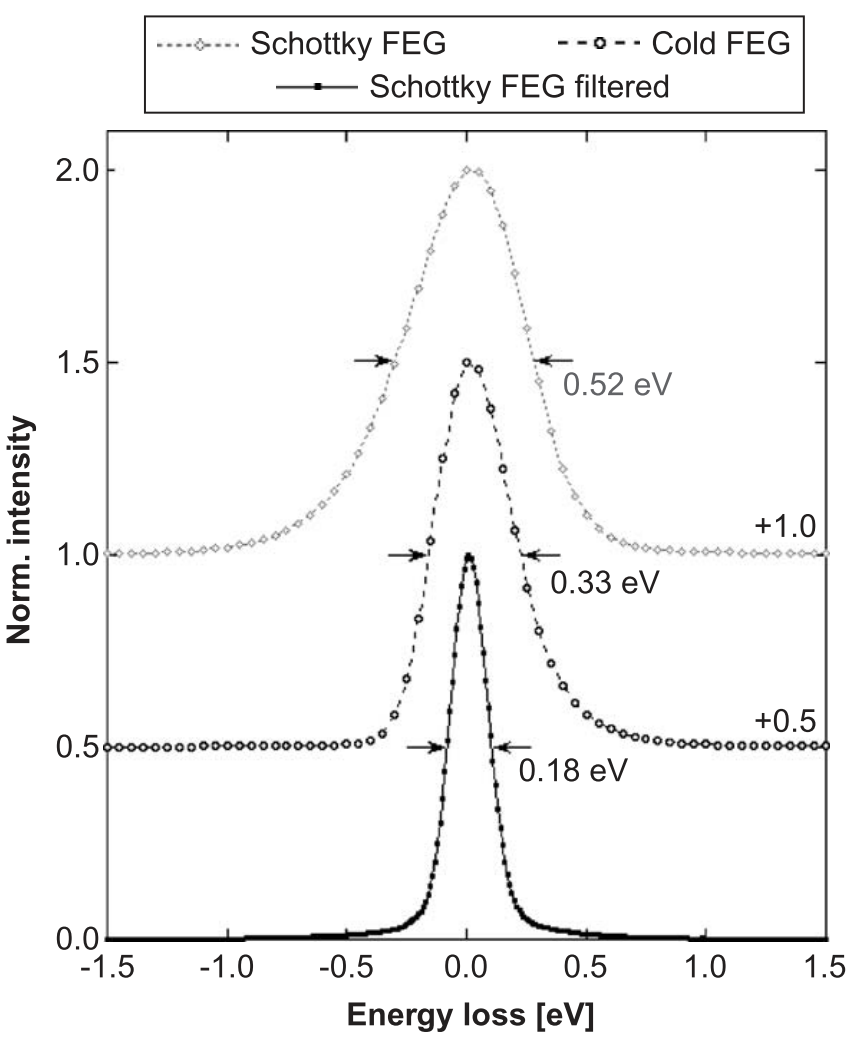
\includegraphics[width=80mm]{plots/monochromator.png}
    \caption{Comparison of the zero-loss peaks of an unfiltered Schottky field emission microscope 
    (200 kV), a cold field-emission microscope (100 kV) and a monochromated electron beam with 
    Schottky field-emission source (200 kV). 
    The second ZLP shows a wider tail at the low-energy side and the tails of the 
    monochromated beam are highly symmetrical. 
    The FWHM indicated in each case provides a measure for the energy resolution.
    %
    Retrieved directly from~\cite{Erni:2005}.}
    \label{fig:monochromation}
\end{figure}


\subsection{ZLP subtraction}
%%%%%%%%%%%
The properties of the ZLP in monochromated EELS depend on the electron energy dispersion,
the monochromator alignment, and the sample thickness~\cite{Park:2008, Stoger:2008}.
%
The first two limitations are already preesent in the absence of a specimen (vacuum operation),
but the third one is associated
to elastic interactions with the sample such as 
phonon excitation, atomic scattering, and exciton losses.
%
This implies that measurements of vacuum EEL spectra can be used for calibration purposes
but not to directly subtract the ZLP from spectra taken on specimens, since their shapes will differ
in general.
%%%%%%%%%%%%%%%


The most important aspect complicating the study of the low-loss regime of EEL spectra 
is the observation of the zero-loss peak, a very intense and ubitiquous feature 
whose right-hand tail suppresses the low-loss features, which results in the loss
of important information within the spectrum.
%
Before analysing the low-loss region of EEL spectra, accurate removal of the
ZLP is crucial. 
%
In the last several years different removal routines for the ZLP were introduced, 
as the increasing energy resolution of the instrumentation would allow for bandgap 
determination by means of VEELS. 
%
The most general suggestion is the subtraction of a fitted ZLP rather than 
using the vacuum recorded ZLP, because a separately recorded peak is always 
different in shape than the one recorded on a sample, due to phonon excitations, 
exciton losses, and broadening at the surface of the sample.
%
Due to the obvious difference in shape between vacuum and in-sample recorded ZLPs, 
direct subtraction of the first on the latter would introduce an extra
source of error. 
%
For this reason, using a fitted ZLP and subtracting it from the EEL spectrum 
is the preferred way to go.
%
Representative examples include the subtraction of a fitted Lorentzian distribution~\cite{Dorneich:1998},
directly subtracting the mirrored left-hand side of the ZLP~\cite{Lazar:2003},
the subtraction of a power-law fit~\cite{Erni:2005}, and the use of a
more general multi-parameter function~\cite{Benthem:2001}.
%
These and several other attempts to model the ZLP distribution 
have had some success at describing the main intensity of the peak, 
but in the tails discrepancies can be as large as several tens of percent~\cite{Bangert:2003}.
%
The standard method for background subtraction of the tails
is to fit a power law to the tails, however this approach is not suitable in
many circumstances~\cite{Hachtel:2018, Tenailleau:1992, Reed:2002, Bosman:2006}.
%
Especially in the very-low-loss region, a simple functional fit completely
removes all intensities belonging to losses within the bandgap energy.
%
More recent studies use integrated software applications for background subtraction 
methods~\cite{Egerton:10.1016/S0304-3991(01)00155-3, Held:2020, Granerod:2018, Fung:2020}.\\

One common flaw of these subtraction methods is the fact that they are often based on specific
model assumptions about the ZLP properties and thereby introduce a methodological
bias which size is difficult to quantify. 
%
This bias arises from assumptions made {\it e.g.} on its functional form, symmetry 
properties, or the fitting range that has been used, all introducing an arbitrariness
to the procedure.
%
Even more importantly, these subtraction methods lack an estimate of the associated uncertainties, 
which in turn affects the reliability of any physical interpretation of features that are observed
in the ZLP-subtracted spectra. 

Developing a model-independent strategy that allows for a determination of the ZLP
with a faithful uncertainty estimate is highly coveted.
%
With the knowledge that the magnitude and shape of the ZLP depend
not only on the specific values
of the electron energy loss $\Delta E$, but also on other operation parameters
of the TEM such as the electron beam energy $E_{\rm b}$, the exposure time
$t_{\rm exp}$, the aperture width and the potential use of a monochromator,
one cannot measure the ZLP for a given operating
condition, for instance a high beam voltage of $E_{\rm b}=200$ keV, and expect to reproduce
the ZLP distribution
associated to different conditions, such as a lower beam voltage of $E_{\rm b}=60$ keV,
without introducing model assumptions.
%
Since it is not possible to compute the dependence of the ZLP on $\Delta E$
and the other operating conditions of the microscope from first principles,
reliance on specific models appears to be unavoidable.
%
Furthermore, even for identical operating conditions, 
the intensity of the ZLP will in general vary due to {\it e.g.} external perturbations 
such as electric or magnetic fields~\cite{Rafferty:2000},
the stability of the microscope and spectrometer electronics~\cite{Kothleitner:2003}, 
the local environment (possibly exposed to mechanical, pressure and temperature fluctuations) 
and spectral aberrations~\cite{Egerton:1996}. 
%
Any model for the ZLP should thus account for this source of uncertainties.

